\documentclass{article}
\usepackage[fleqn]{amsmath}
\usepackage{amssymb}
\usepackage{enumitem}
\usepackage{amsthm}
\usepackage{mystyle}
\usepackage{hyperref}
\usepackage[margin=1in]{geometry}
\usepackage{float}
\usepackage{graphicx}
\usepackage[
backend=biber,
style=alphabetic
]{biblatex}
\addbibresource{references.bib}


\geometry{outer=2cm}

\title{How robust are traditional stock price models under bubble-like market dynamics?\\Analysis of the AI bubble}
\author{Mya Mokrane\\McGill University\\261104994}
\date{May 18, 2026}

\begin{document}
\maketitle
\tableofcontents 


\section*{Abstract}

The AI bubble.

HELLOOOO


\newpage

\section*{Introduction}
\addcontentsline{toc}{section}{Introduction}

  The rapid development of artificial intelligence has had a profound impact not only on daily life and future labor markets, but also on global financial markets and large technological enterprises. Artificial intelligence has evolved beyond a simple computational tool and has become increasingly integrated into research, scientific experimentation, optimization, and large-scale decision-making processes used by both corporations and governments.

  As a result, investment in artificial intelligence technologies and infrastructure has grown dramatically over the past decade. In particular, the extraordinary increase in demand for AI services, cloud computing, and semiconductor technology has led to substantial growth in the market valuations of AI-focused firms. This rapid appreciation in stock prices has raised concerns regarding the possible formation of speculative bubbles within AI-related assets.
  
  Major technology companies such as NVIDIA, Meta Platforms, and Microsoft have experienced exceptional increases in their stock prices during the post-pandemic period, particularly following the emergence of large-scale generative AI systems.

This naturally raises the following question: to what extent can traditional financial models remain relevant in describing or predicting the dynamics of AI-related equities during speculative market periods?

Among the most influential classical financial models is the Black--Scholes framework, developed in 1973, which introduced one of the most widely used option pricing formulas in quantitative finance. The model assumes that stock prices follow a geometric Brownian motion with constant volatility and continuous dynamics.

  \begin{figure}[H]
    \centering
    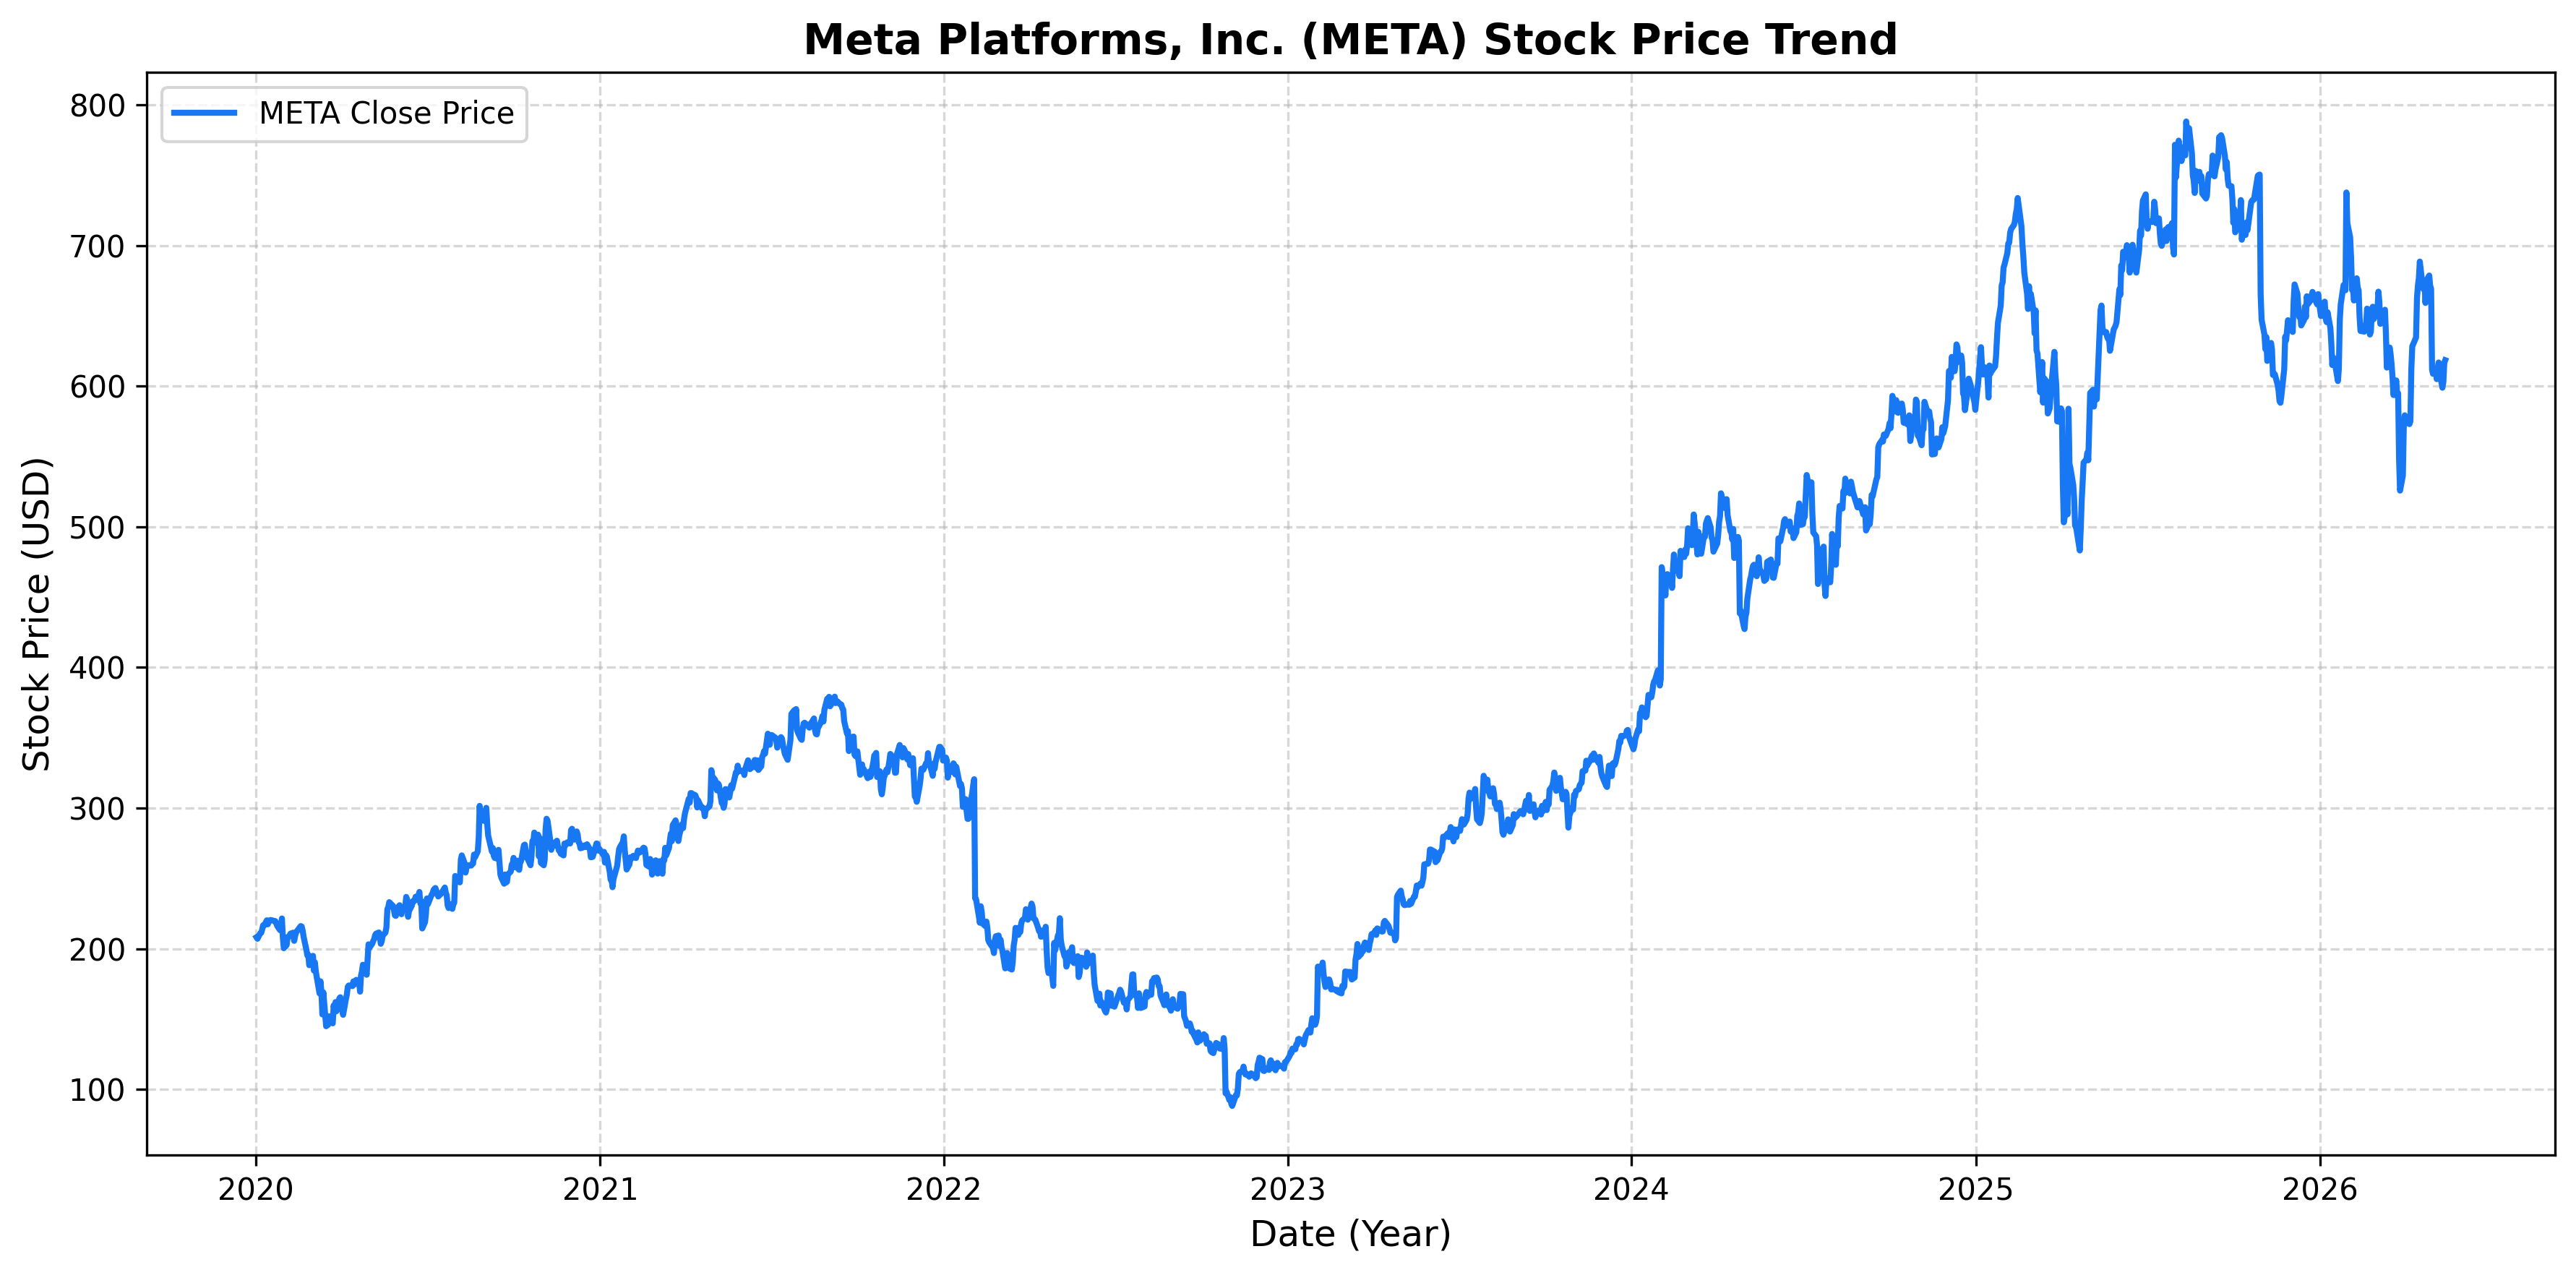
\includegraphics[width=0.8\textwidth]{../figures/meta_close_price.png}
    \caption{META closing stock price since 2020.}
    \label{fig:meta_price}
  \end{figure}

  As illustrated in Figure~\ref{fig:meta_price}, META experienced substantial volatility during the post-pandemic AI expansion period. Such behavior raises important questions regarding the suitability of traditional diffusion-based models under highly speculative market conditions characterized by volatility clustering, rapid price appreciation, and abrupt market corrections.

  This paper investigates whether classical stochastic models such as Black--Scholes remain informative in the context of AI-related equities, and explores the extent to which more advanced models incorporating stochastic volatility or jump dynamics may better capture the statistical behavior of speculative assets.

\section*{Black-Scholes Model}
\addcontentsline{toc}{section}{Black-Scholes Model}

\subsection{Black-Scholes Formula for Option Pricing}
 In 1973, Fisher Black and Myron Scholes published their groundbreaking work option pricing. Indeed, in their article "The Pricing of Options and Corporate Liabilities" \cite{black1973pricing}, they derived the Black-Scholes formula for option pricing:
 \begin{equation}
    C^{BS}(t, S; r, \sigma, K, T) := S \Phi(d_1) - K e^{-r(T-t)} \Phi(d_2)
    \label{Black-Scholes Equation}
 \end{equation}
 where $\Phi$ denotes the standard normal distribution (df), $r$ represents the continuously compounded risk -free interest rate, $\sigma$ denotes the volatility of the underlying stock, and where 
  $$d_1 = \frac{\ln\frac{S}{K} + (r+\frac{1}{2}\sigma^2)(T-t)}{\sigma \sqrt{T-t}} \qquad d_2 = d_1 - \sigma \sqrt{T-t}$$

  Here, $K$ is the premium, while T is the maturity of the option. 

  We will use standard market practices where time is measured in years and $r$ and $\sigma$ are expressed in annualized terms.

  Furthermore, we will set $S_t$ to be the price of the stock at time $t$. Real market insterest rates and volatitilities change constanstly and thus depend on time : $ r_t, \sigma_t$. As a result, we take the vector of risk-factors as a function of time: $\textbf{Z}_t = (\ln S_t, r_t, \sigma_t)'$.

  The risk-factor changes are given by : 
  \begin{equation}
    \textbf{X}_{t+1} = (\ln S_{t+1} - \ln S_t, r_{t+1}-r_t, \sigma_{t+1} - \sigma_t)'.
    \label{BS: Risk-Factor Changes}
  \end{equation}

  \subsection{Geometric Brownian Motion for Stock Prices}

  \begin{figure}[H]
    \centering
    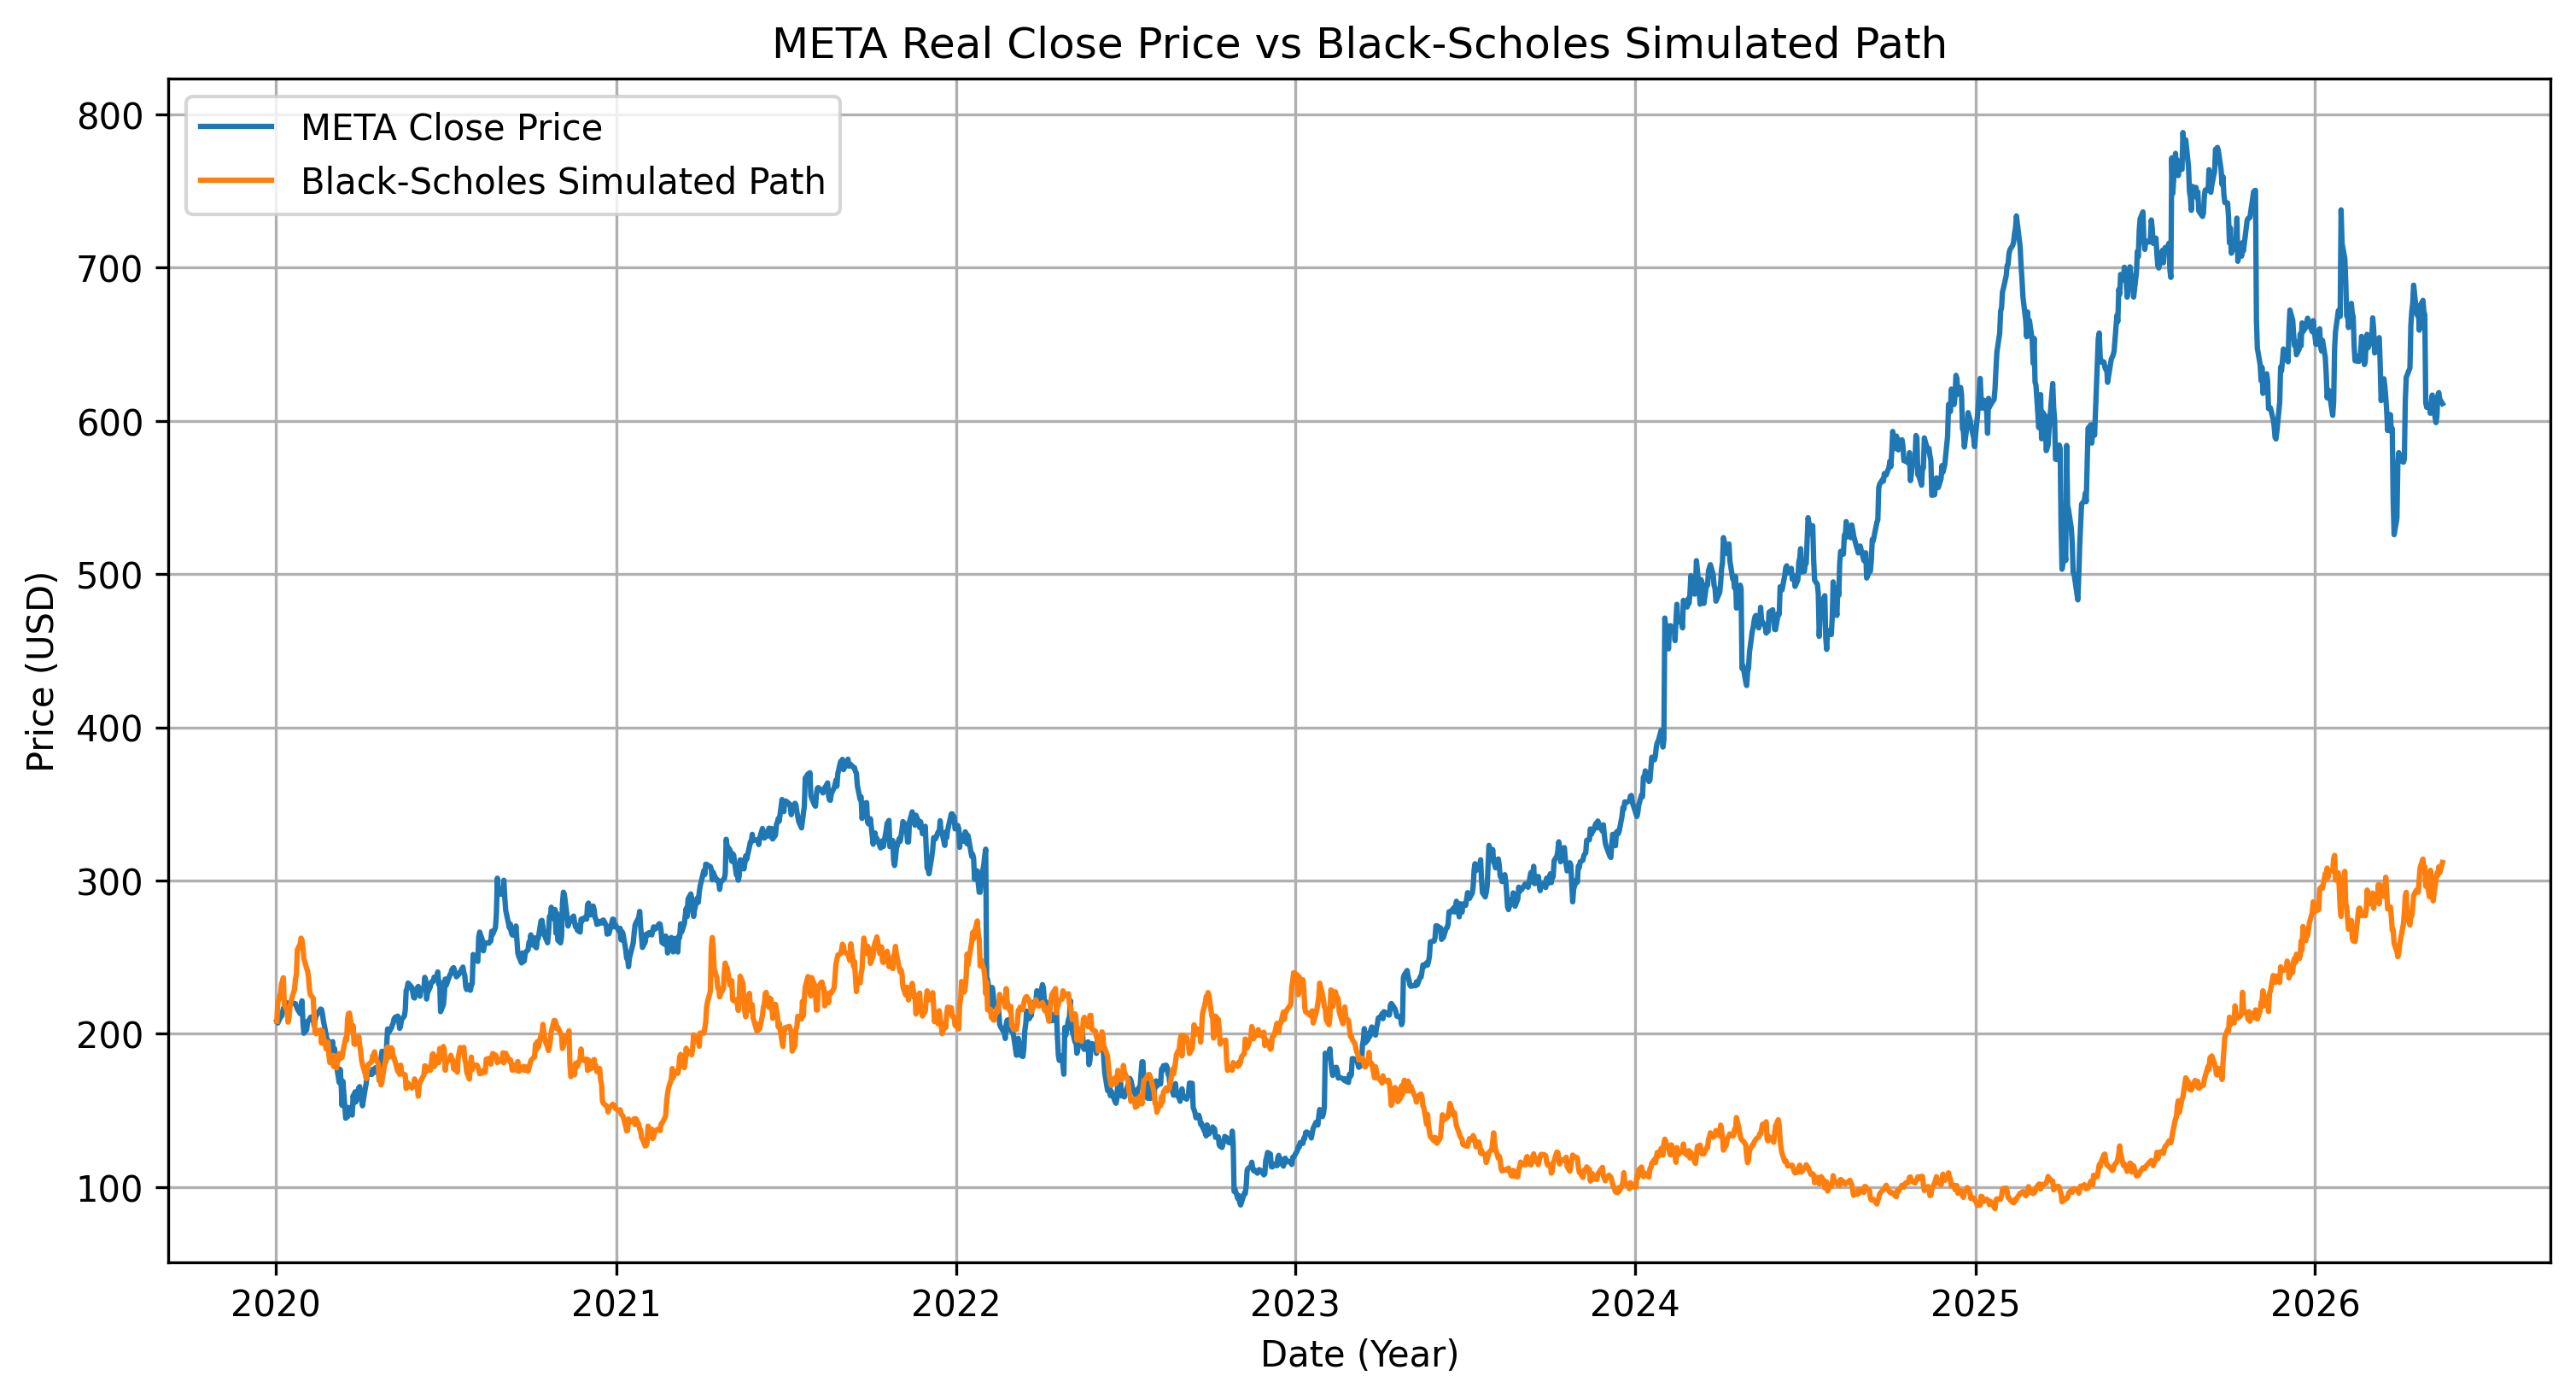
\includegraphics[width=0.8\textwidth]{../figures/meta_close_price_vs_BS_path.png}
    \caption{META closing stock price vs Black Scholes Simulated path since 2020.}
    \label{fig:meta_BS_price}
  \end{figure}

\section*{New Methods}
\addcontentsline{toc}{section}{New Methods}

\subsection*{Times Series Analysis : GARCH Model}


\subsection*{AI Stress-Testing}



\printbibliography

\end{document}